\documentclass[11pt]{article}

\usepackage[margin=1in]{geometry}
\usepackage{amsmath,amssymb,amsthm}
\usepackage{graphicx}
\usepackage{hyperref}

\newtheorem{theorem}{Theorem}
\newtheorem{lemma}{Lemma}
\newtheorem{remark}{Remark}

\newcommand{\C}{\mathbb C}
\newcommand{\re}{\operatorname{Re}}
\newcommand{\Tr}{\operatorname{Tr}}
\newcommand{\diag}{\operatorname{diag}}
\newcommand{\dist}{\operatorname{dist}}
\newcommand{\rank}{\operatorname{rank}}
\newcommand{\norm}[1]{\left\lVert #1 \right\rVert}
\newcommand{\eps}{\varepsilon}
\newcommand{\PiX}{\Pi(X)}

\title{The Bishop-Phelps-Bollobas Moduli of \(M_2(\mathbb C)\) Are Maximal}
\author{FA/Banach discovery run \texttt{fa\_banach\_001}}
\date{2026-06-20}

\begin{document}
\maketitle

\section*{Source Question}

The source paper is Chica--Kadets--Martin--Moreno-Pulido--Rambla-Barreno,
\emph{Bishop-Phelps-Bollobas moduli of a Banach space}, arXiv:1304.0376.
It proves that many Banach spaces have maximal Bishop-Phelps-Bollobas
moduli, including unital \(C^*\)-algebras with nontrivial center, and then
raises the case of \(L(H)\), where those centralizer methods do not apply.

\begin{center}
\IfFileExists{figures/source_discussion_crop.png}{%
  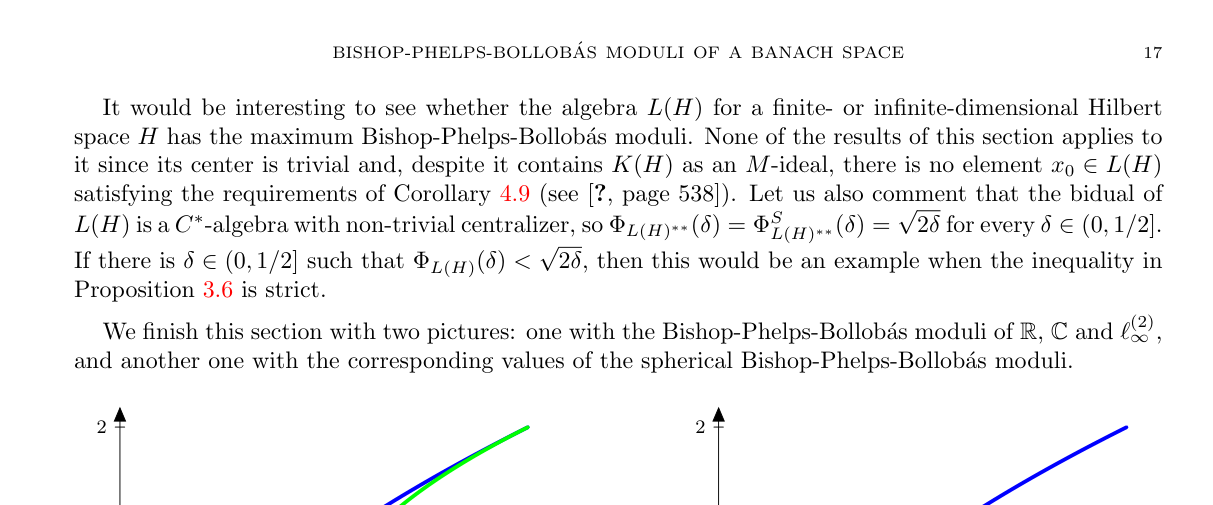
\includegraphics[width=0.90\linewidth]{figures/source_discussion_crop.png}
}{}
\end{center}

This packet proves the first noncentral Hilbert-operator case:
\[
  L(\mathbb C^2)=M_2(\mathbb C).
\]
It does not solve the higher-dimensional or infinite-dimensional \(L(H)\)
problem.

\section*{Definitions}

For a Banach space \(X\), write
\[
  \Pi(X)=\{(y,y^*)\in S_X\times S_{X^*}: y^*(y)=1\}.
\]
The Bishop-Phelps-Bollobas modulus \(\Phi_X(\delta)\) is the least radius
which approximates every pair \((x,x^*)\in B_X\times B_{X^*}\) satisfying
\(\re x^*(x)>1-\delta\) by some element of \(\Pi(X)\). The spherical
modulus \(\Phi_X^S(\delta)\) is defined in the same way but only for
\((x,x^*)\in S_X\times S_{X^*}\).

The source paper proves the universal bound
\[
  \Phi_X^S(\delta)\leq \Phi_X(\delta)\leq \sqrt{2\delta}
  \qquad (0<\delta<2)
\]
and also proves that \(\Phi_X(\delta)=\sqrt{2\delta}\) if and only if
\(\Phi_X^S(\delta)=\sqrt{2\delta}\). We only need the upper bound and the
obvious implication from a spherical lower bound to an ordinary lower bound.

We identify \(M_2(\mathbb C)^*\) with \(S_1^2\), the trace-norm class, by
\[
  T(a)=\Tr(Ta), \qquad \norm{T}_{(M_2)^*}=\norm{T}_1 .
\]

\section*{Theorem}

\begin{theorem}
Let \(X=M_2(\mathbb C)\) with the operator norm. Then
\[
  \Phi_X(\delta)=\Phi_X^S(\delta)=\sqrt{2\delta}
  \qquad (0<\delta\leq 1/2).
\]
\end{theorem}

\section*{Proof}

We first record the trace-norm obstruction.

\begin{lemma}\label{lem:rank-one-distance}
Let \(0<\eps\leq1\), put
\[
  x=\diag(1-\eps,1),\qquad
  \rho=\diag(\eps/2,1-\eps/2).
\]
If \((y,T)\in \Pi(M_2(\mathbb C))\), then
\[
  \max\{\norm{x-y},\norm{\rho-T}_1\}\geq \eps .
\]
\end{lemma}

\begin{proof}
Let \((y,T)\in\Pi(M_2(\mathbb C))\), so
\[
  \norm{y}=1,\qquad \norm{T}_1=1,\qquad \Tr(Ty)=1.
\]
If \(\norm{x-y}\geq\eps\), there is nothing to prove. Assume from now on
that \(\norm{x-y}<\eps\).

First, \(y\) is not unitary. Indeed, for every unitary \(u\),
\[
  \norm{x-u}\geq \norm{xe_1-ue_1}
  \geq \bigl|\norm{ue_1}-\norm{xe_1}\bigr|
  =1-(1-\eps)=\eps .
\]
Thus \(\norm{x-y}<\eps\) excludes unitary \(y\).

Since \(y\) is a nonunitary \(2\times2\) contraction of norm one, its
singular values are \(1\) and \(s\), where \(0\leq s<1\). Choose a singular
value decomposition
\[
  y=U\diag(1,s)V^* .
\]
Set \(S=V^*TU\). Then \(\norm{S}_1=1\) and, by cyclicity of the trace,
\[
  1=\Tr(Ty)=\Tr(S\diag(1,s)).
\]
Writing \(S=(s_{ij})\), we get
\[
  1=\left|s_{11}+s\,s_{22}\right|
  \leq |s_{11}|+s|s_{22}|
  \leq |s_{11}|+|s_{22}|
  \leq \norm{S}_1=1.
\]
Because \(s<1\), equality forces \(s_{22}=0\) and \(|s_{11}|=1\). The
trace norm dominates the Hilbert-Schmidt norm, so
\[
  1=\norm{S}_1\geq \norm{S}_2
  =\left(|s_{11}|^2+|s_{12}|^2+|s_{21}|^2+|s_{22}|^2\right)^{1/2}.
\]
Since \(|s_{11}|=1\), this gives \(s_{12}=s_{21}=0\). Hence
\(S=\diag(1,0)\), after the phase is fixed by
\(\Tr(S\diag(1,s))=1\), and therefore \(T\) is rank one.

Now compare \(\rho\) with rank-one trace-norm-one matrices. The singular
values of \(\rho\) are \(1-\eps/2\) and \(\eps/2\), while the singular
values of any rank-one \(T\) with \(\norm{T}_1=1\) are \(1\) and \(0\).
The Ky Fan--Mirsky singular-value inequality gives
\[
  \norm{\rho-T}_1
  \geq \left|(1-\eps/2)-1\right|+\left|\eps/2-0\right|
  =\eps .
\]
Therefore, if \(\norm{x-y}<\eps\), then \(\norm{\rho-T}_1\geq\eps\). This
proves the lemma.
\end{proof}

We now prove the theorem. Fix \(0<\delta\leq1/2\). Let \(0<\gamma<\delta\)
and set \(\eps=\sqrt{2\gamma}\). Since \(\gamma<\delta\leq1/2\), we have
\(0<\eps\leq1\). With \(x\) and \(\rho\) as in Lemma~\ref{lem:rank-one-distance},
\[
  \norm{x}=1,\qquad \norm{\rho}_1=1,
\]
and
\[
  \Tr(\rho x)
  =(\eps/2)(1-\eps)+(1-\eps/2)
  =1-\eps^2/2
  =1-\gamma
  >1-\delta .
\]
Thus \((x,\rho)\) is an admissible spherical test pair for
\(\Phi_X^S(\delta)\). Lemma~\ref{lem:rank-one-distance} says that its
\(d_\infty\)-distance to \(\Pi(X)\) is at least \(\eps=\sqrt{2\gamma}\).
Hence
\[
  \Phi_X^S(\delta)\geq \sqrt{2\gamma}.
\]
Letting \(\gamma\uparrow\delta\), we obtain
\[
  \Phi_X^S(\delta)\geq\sqrt{2\delta}.
\]
The universal upper bound gives
\[
  \Phi_X^S(\delta)\leq\Phi_X(\delta)\leq\sqrt{2\delta}.
\]
Therefore both moduli are equal to \(\sqrt{2\delta}\).

\section*{Limitations and Next Target}

This proof is genuinely two-dimensional. The step ``\(y\) is nonunitary,
hence the top singular subspace is one-dimensional'' fails in \(M_n\) for
\(n\geq3\): a nonunitary norm-one contraction may still have a large
singular subspace for singular value \(1\). The higher-dimensional
noncentral-projection route would need to control norming trace-class
functionals supported on that larger top singular face.

Thus this packet gives a verified base case for the source paper's
\(L(H)\) question, not the full answer for finite-dimensional \(H\) nor for
infinite-dimensional \(B(H)\).

\begin{thebibliography}{9}

\bibitem{CKMMR2013}
M. Chica, V. Kadets, M. Martin, S. Moreno-Pulido and F. Rambla-Barreno,
\emph{Bishop-Phelps-Bollobas moduli of a Banach space},
J. Math. Anal. Appl. 412 (2014), 697--719; arXiv:1304.0376.

\bibitem{Bhatia1997}
R. Bhatia,
\emph{Matrix Analysis},
Graduate Texts in Mathematics 169, Springer, 1997.

\end{thebibliography}

\end{document}
